\subsection*{Problema 15}
\textbf{Enunciado:} Evaluar la integral definida mediante sumas de Riemann:
\begin{align*}
\int_{0}^{\pi} \cos x \, dx
\end{align*}

\textbf{Solución:}
Para evaluar la integral mediante la definición de la suma de Riemann, utilizamos el límite por la derecha con una partición regular de $[0, \pi]$ en $n$ subintervalos de ancho:
\begin{align*}
\Delta x = \dfrac{\pi - 0}{n} = \dfrac{\pi}{n}
\end{align*}

Los puntos de la partición se definen como $x_i = i \Delta x = \dfrac{i\pi}{n}$ para $i = 1, 2, \dots, n$. Evaluamos la función en los extremos derechos:
\begin{align*}
f(x_i) = \cos\left(\dfrac{i\pi}{n}\right)
\end{align*}

La integral definida se plantea como el límite de la suma de Riemann:
\begin{align*}
\int_{0}^{\pi} \cos x \, dx &= \lim_{n \to \infty} \sum_{i=1}^n f(x_i)\Delta x \\
&= \lim_{n \to \infty} \dfrac{\pi}{n} \sum_{i=1}^n \cos\left(\dfrac{i\pi}{n}\right)
\end{align*}

Para calcular la suma de cosenos, empleamos la identidad trigonométrica estándar para progresión aritmética:
\begin{align*}
\sum_{i=1}^n \cos(i\theta) = \dfrac{\sin\left(\frac{n\theta}{2}\right)\cos\left(\frac{(n+1)\theta}{2}\right)}{\sin\left(\frac{\theta}{2}\right)}
\end{align*}

Sustituyendo $\theta = \Delta x = \dfrac{\pi}{n}$, el numerador del argumento del seno se convierte en $\dfrac{n\theta}{2} = \dfrac{\pi}{2}$. La suma resulta en:
\begin{align*}
\sum_{i=1}^n \cos\left(\dfrac{i\pi}{n}\right) &= \dfrac{\sin\left(\frac{\pi}{2}\right)\cos\left(\frac{(n+1)\pi}{2n}\right)}{\sin\left(\frac{\pi}{2n}\right)} \\
&= \dfrac{1 \cdot \cos\left(\frac{\pi}{2} + \frac{\pi}{2n}\right)}{\sin\left(\frac{\pi}{2n}\right)}
\end{align*}

Utilizando la identidad $\cos\left(\frac{\pi}{2} + \alpha\right) = -\sin(\alpha)$, simplificamos el numerador:
\begin{align*}
\cos\left(\frac{\pi}{2} + \frac{\pi}{2n}\right) = -\sin\left(\frac{\pi}{2n}\right)
\end{align*}

Por lo tanto, la suma se reduce a:
\begin{align*}
\sum_{i=1}^n \cos\left(\dfrac{i\pi}{n}\right) = \dfrac{-\sin\left(\frac{\pi}{2n}\right)}{\sin\left(\frac{\pi}{2n}\right)} = -1
\end{align*}

Sustituimos este resultado en el límite de la integral:
\begin{align*}
\int_{0}^{\pi} \cos x \, dx &= \lim_{n \to \infty} \dfrac{\pi}{n} (-1) \\
&= \lim_{n \to \infty} \left( -\dfrac{\pi}{n} \right) = 0
\end{align*}

El valor de la integral definida es $0$.

\begin{figure}[H]
	\centering
	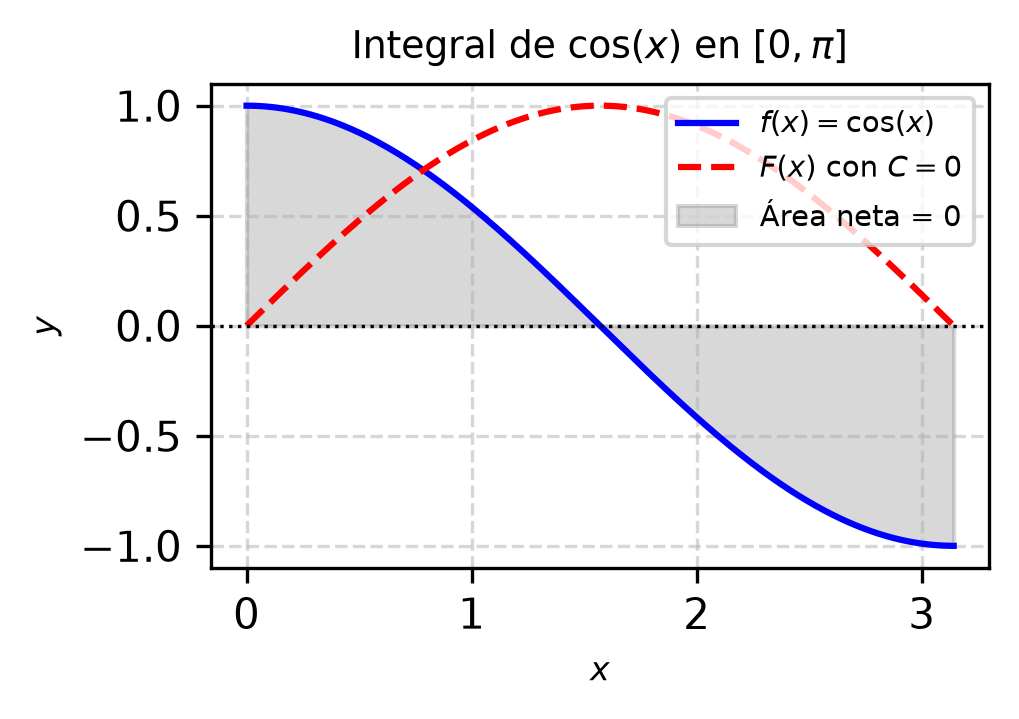
\includegraphics[width=\columnwidth]{semana_06/graficas/SEM06_P15_grafica.png}
	\caption{Representación gráfica de $f(x)$ y su antiderivada $F(x)$ evaluada para la constante de integración $C = 0$ (Problema 15).}
	\label{fig:problema15}
\end{figure}
